\documentclass{article}
\usepackage[margin=1in]{geometry} % For setting page margins
\usepackage{amsmath}
\usepackage{amssymb} % For math symbols and equations
\usepackage{graphicx} % For including images
\usepackage{hyperref} 
\usepackage{enumitem}
\usepackage{float}
\usepackage{listings}
\usepackage{xcolor}
\usepackage{caption}

\renewcommand{\thesection}{\arabic{section}.}
\renewcommand{\thesubsection}{(\alph{subsection})}

\lstdefinestyle{matlabstyle}{
    language=Matlab,              % Specify the language
    basicstyle=\ttfamily\footnotesize\color{black}, % Code font
    keywordstyle=\color{blue}\bfseries, % Keywords in blue
    stringstyle=\color{orange},    % Strings in green
    commentstyle=\color{magenta}, % Comments in magenta
    numbers=left,                 % Line numbers on the left
    numberstyle=\tiny\color{black},% Line number style
    stepnumber=1,                 % Line number increment
    breaklines=true,              % Line breaking
    frame=single,                 % Border around code
    backgroundcolor=\color{white},
    tabsize=4,                    % Tab size
    showstringspaces=false,       % Don't show spaces in strings
}

\begin{document}

\title{
    \begin{tabular}{@{}l@{}}
        \textbf{Class:} Robust Multivariate Control \\
        \textbf{Professor:} Dr. Sean Humbert \\
        \textbf{TAs:} Santosh Chaganti \\
        \textbf{Student:} Steve Gillet \\
        \textbf{Date:} \today \\
        \textbf{Assignment:} Homework 7
    \end{tabular}
}

\author{}
\date{}

\maketitle

\section{}
\textit{For the following MIMO uncertainty models, sketch the block diagram and transform the standard $G$ and $K$ feedback system into the $M \Delta$ structure and determine $M$, and apply the Small Gain Theorem to find the associated robust stability test:}

\subsection{}
\textit{$\tilde{G}=\left(I+\Delta W_o\right) G \quad$ (Multiplicative Output)}

The block diagram looks like this:

\begin{figure}[H]
    \centering
    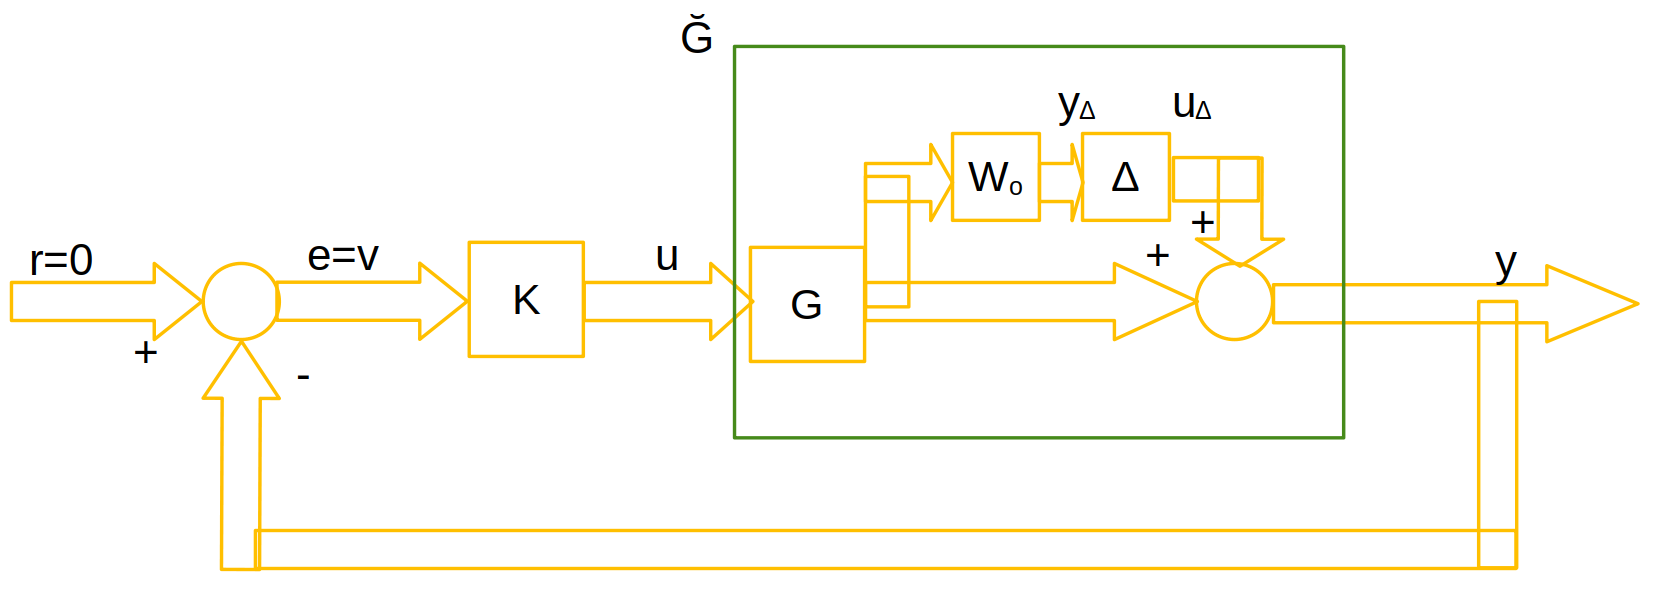
\includegraphics[width=\textwidth]{1aDiagram.png}
    \caption{Multiplicative Output Uncertainty Block Diagram}
    \label{fig:1aDiagram}
\end{figure}

The $M \Delta$ structure is as follows:

\begin{figure}[H]
    \centering
    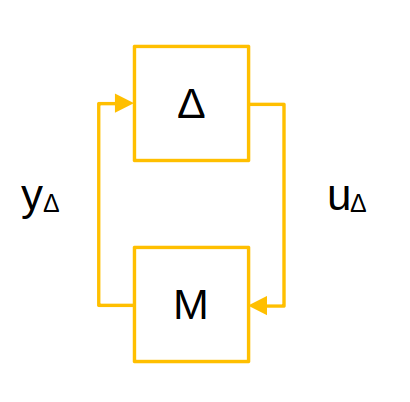
\includegraphics[width=0.5\textwidth]{mDeltaDiagram.png}
    \caption{M-$\Delta$ Diagram}
    \label{fig:mDeltaDiagram1}
\end{figure}

$y_\Delta = Mu_\Delta$

Applying Small Gain Theorem to get M and the Robust Stability test:

\begin{align}
    y_\Delta &= -K G W_o y \\
    y &= -GKy+u_\Delta \\
    y &= -(I + GK)^{-1} u_\Delta \\
    y_\Delta &= -K G W_o S_o u_\Delta \\
    M &= -T_o W_o
\end{align}

Robust Stability Test:

$\| W_o T_o G\|_\infty < 1$

\subsection{}
\textit{$\tilde{G}=G\left(I-W_i \Delta\right)^{-1} \quad$ (Inverse Multiplicative Input)}

The block diagram looks like this:

\begin{figure}[H]
    \centering
    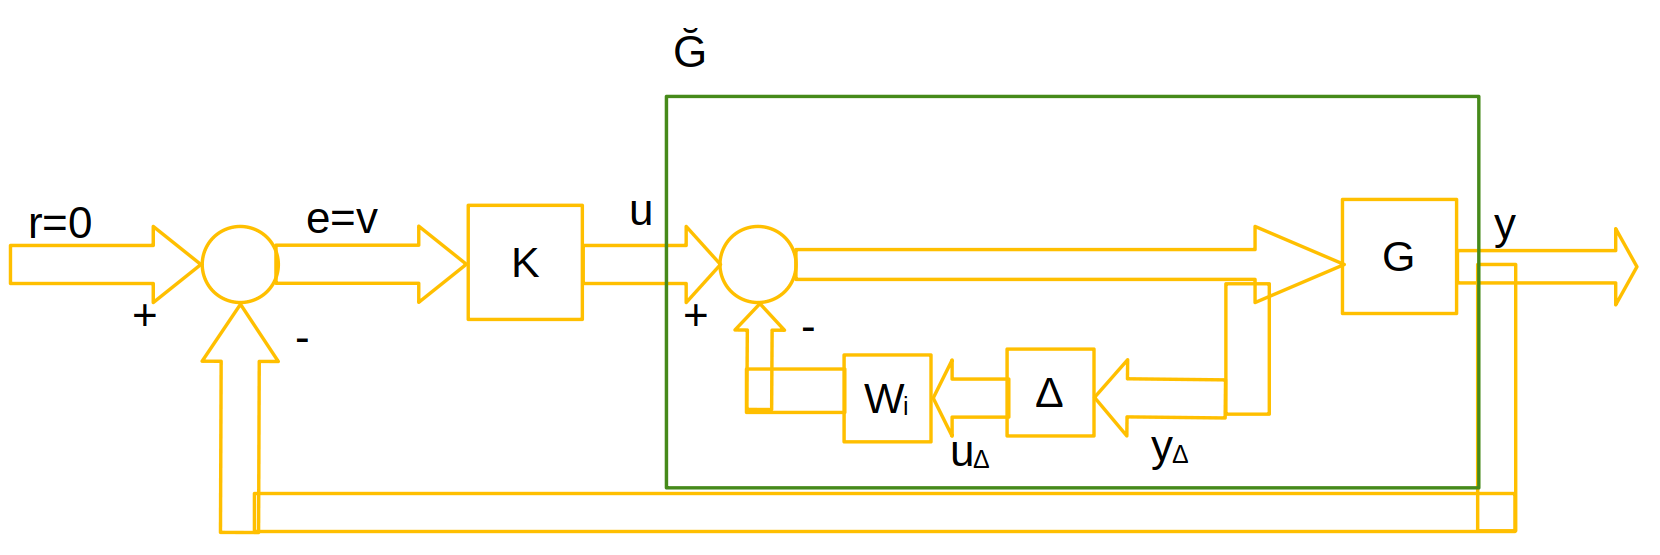
\includegraphics[width=\textwidth]{1bDiagram.png}
    \caption{Inverse Multiplicative Input Uncertainty Block Diagram}
    \label{fig:1bDiagram}
\end{figure}

The $M \Delta$ structure is as follows:

\begin{figure}[H]
    \centering
    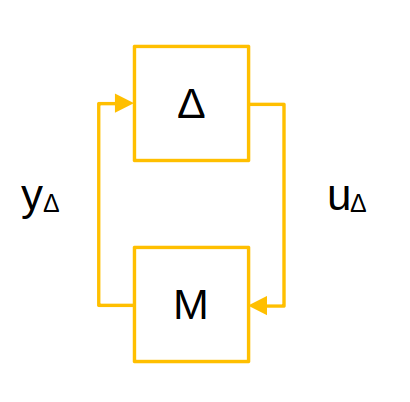
\includegraphics[width=0.5\textwidth]{mDeltaDiagram.png}
    \caption{M-$\Delta$ Diagram}
    \label{fig:mDeltaDiagram2}
\end{figure}

$y_\Delta = Mu_\Delta$

Applying Small Gain Theorem to get M and the Robust Stability test:

\begin{align}
    y_\Delta &=-Ky \\
    y &= G(-Ky-W_i u_\Delta) \\
    y &= (I + GK)^{-1}G W_i u_\Delta \\
    y_\Delta &= -K S_o G W_i u_\Delta \\
    M &= -K S_o G W_i
\end{align}

Robust Stability Test:

$\| S_o G W_i \|_\infty < 1$

\section{}
\textit{For the following MIMO plant and controller,
\[
G(s)=\left(\begin{array}{cc}
\frac{2}{s+1} & \frac{1}{(s+1)(s+2)} \\
\frac{1}{(s+1)(s+2)} & \frac{2}{s+2}
\end{array}\right), \quad K(s)=\left(\begin{array}{cc}
\frac{2}{s+2} & 0 \\
0 & \frac{1}{s+3}
\end{array}\right),
\]}

\subsection{}
\textit{Generate singular value bode plots for $G, T_o$, and $S_o\left(=S_I\right.$ in this case) and label the min and max singular values. The MATLAB command sigma will be useful here.}

\begin{figure}[H]
    \centering
    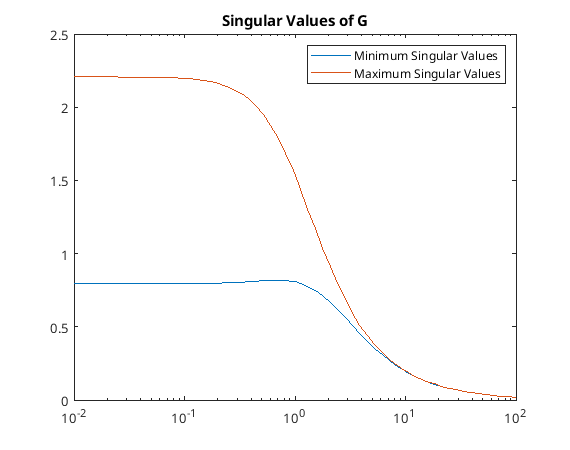
\includegraphics[width=0.75\textwidth]{svG.png}
    \label{fig:svG}
\end{figure}

\begin{figure}[H]
    \centering
    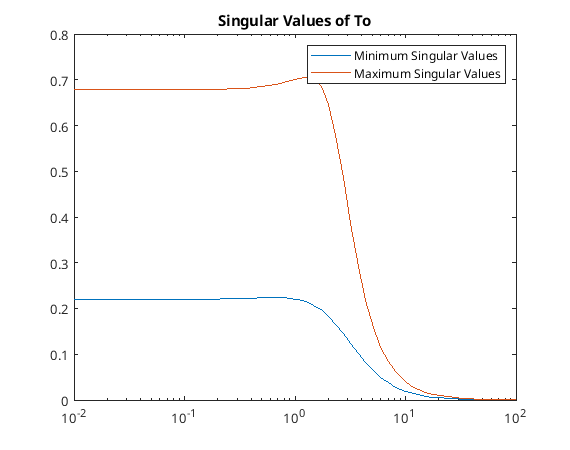
\includegraphics[width=0.75\textwidth]{svTo.png}
    \label{fig:svTo}
\end{figure}

\begin{figure}[H]
    \centering
    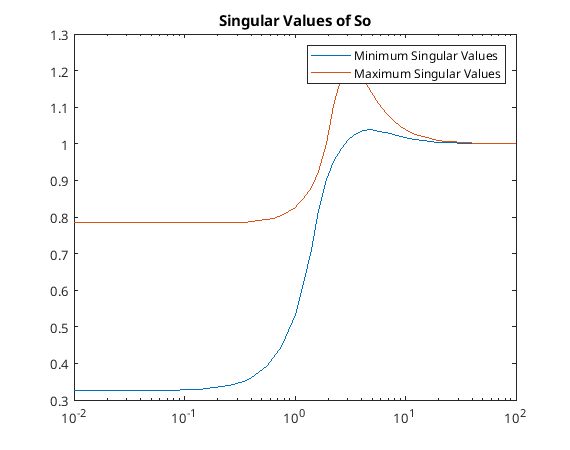
\includegraphics[width=0.75\textwidth]{svSo.png}
    \label{fig:svSo}
\end{figure}

\subsection{}
\textit{What percentage of tracking error would we expect for signals up to $0.1 \mathrm{rad/s}$ for a unity negative feedback system?}

At 0.1 rad/s, the maximum singular value of So is 0.784076, so we would expect a tracking error of 78 \%.

\subsection{}
\textit{For $10 \mathrm{rad/s}$ and above, what level of noise attenuation would we expect this plant to provide at the output for a unity negative feedback system? Recall a gain of 0.1 corresponds to a $10 \mathrm{X}$ reduction.}

At 10 rad/s the maximum singular value of To is 0.0405892, so we would expect a noise attenuation of 24.6X.

\subsection{}
\textit{Determine the minimum perturbation level $\|\Delta\|_{\infty} \leq \gamma$ and frequency that destabilizes the system for multiplicative output uncertainty and inverse multiplicative input uncertainty (assume the weights are identity).}

Found the minimum perturbation levels using the 'sigma' Matlab function to get the $H_\infty$ norm and then taking the inverse:

\begin{lstlisting}[style=matlabstyle]
Mout = -To;
Min = -K*So*G;
gammaOut = norm(Mout, inf);
gammaIn = norm(Min, inf);

[svMout, wMout] = sigma(Mout);
[svMoutMax, iOut] = max(svMout(1,:));
freqOut = wMout(iOut);

disp(1/gammaOut);
disp(freqOut);

[svMin, wMin] = sigma(Min);
[svMinMax, iIn] = max(svMin(1,:));
freqIn = wMin(iIn);

disp(1/gammaIn);
disp(freqIn);
\end{lstlisting}

Results: \\
Multiplicative Output Uncertainty: \\
$\gamma = 1.42047120633257$ \\
$frequency = 1.25918050421322 rad/s$ \\

Inverse Multiplicative Input Uncertainty: \\
$\gamma = 1.42048907280403$ \\ 
$frequency = 1.18617940816049 rad/s$ \\

\section{}
\textit{Consider the MIMO controller and plant:
\[
G(s)=\frac{1}{\tau s+1}\left(\begin{array}{cc}
-87.8 & 1.4 \\
-108.2 & -1.4
\end{array}\right), \quad K(s)=\frac{\tau s+1}{s}\left(\begin{array}{cc}
-0.0015 & 0 \\
0 & -0.075
\end{array}\right)
\]
Assume a time constant $\tau=50$.}

\subsection{}
\textit{Assume the uncertainty in the two channels can be represented using a multiplicative output uncertainty model. The first channel (weight $W_1(s)$) has a $10\%$ error at low frequency, increases to $100\%$ at $10 \mathrm{rad/s}$, and reaches $120\%$ (1.2X) at the high frequency range. The corresponding MATLAB command to generate the first order weight for this channel is $W1 = \text{makeweight}(0.1,10,1.2)$. Similarly, the second channel (weight $W_2(s)$) has a $5\%$ error at low frequency, increases to $100\%$ at $50 \mathrm{rad/s}$, and reaches $150\%$ (1.5X) at the high frequency range. Generate magnitude plots of the two weighting functions (in absolute units, not dB) and label them on the same graph (using bodeplot or sigmaplot with appropriate plot options specified).}

\begin{figure}[H]
    \centering
    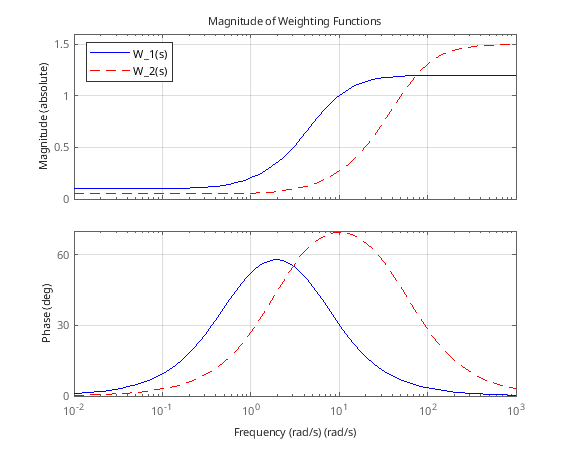
\includegraphics[width=0.75\textwidth]{weightingFunctionsPlot.png}
    \label{fig:weightingFunctionsPlot}
\end{figure}

\subsection{}
\textit{Assume these weights can be represented by the block diagonal weighting matrix
\[
W(s)=\left[\begin{array}{cc}
W_1(s) & 0 \\
0 & W_2(s)
\end{array}\right]
\]
and check to determine whether or not the system is robust with respect to (a) multiplicative output uncertainty, and (b) inverse multiplicative input uncertainty. Be sure to generate the singular value plots in absolute units as a function of frequency (using the MATLAB command sigmaplot). Also compute the robustness margin $\beta$ for each case.}

The multiplicative output uncertainty norm is 0.234 and is therefore robust.
The beta is 4.27.

The inverse multiplicative input uncertainty norm is 0.236 and is therefore robust.
The beta is 4.22.

\begin{figure}[H]
    \centering
    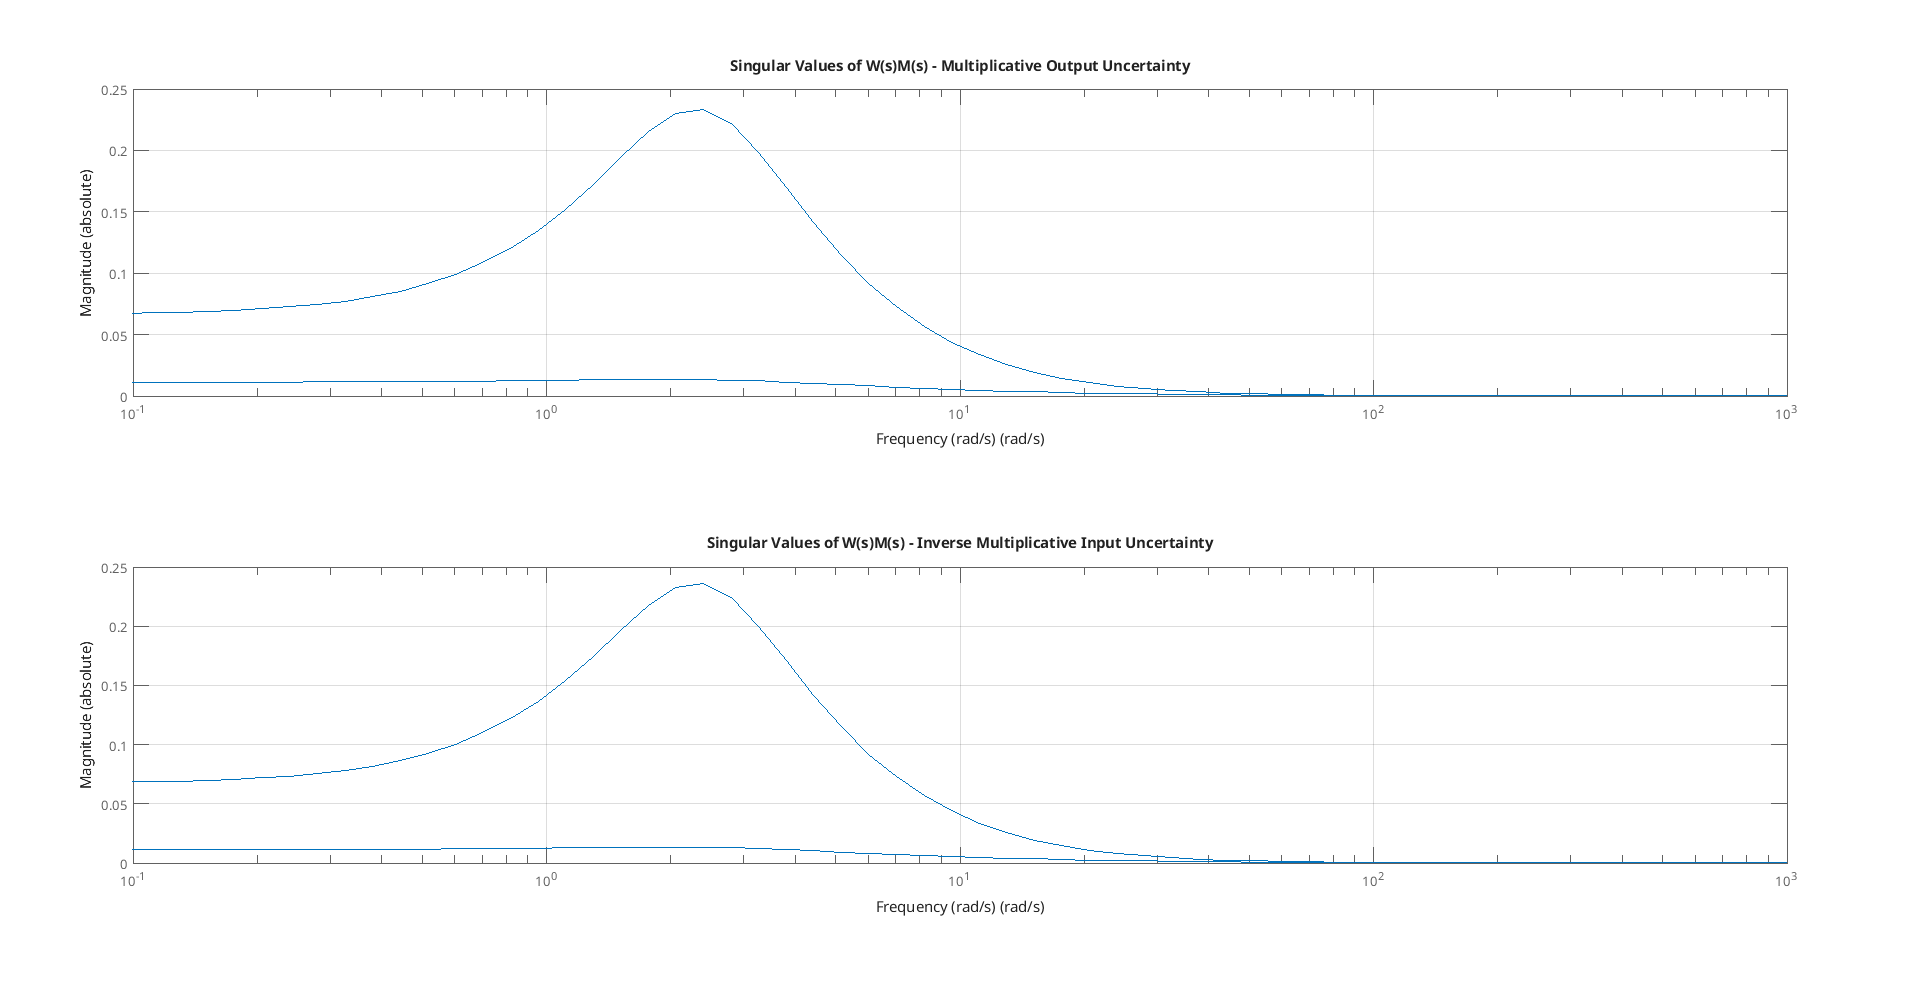
\includegraphics[width=\textwidth]{weightedUncertaintyPlot.png}
    \label{fig:weightedUncertaintyPlot}
\end{figure}

\end{document}